\subsection{k-Ladder Side-Tuning (k-LST)}

In an attempt to close the performance gap for memory efficient PEFT, we introduce k-Ladder Side-Tuning (k-LST). This is a generalization of Ladder Side-Tuning (LST) \cite{sung2022lst}, where LST can be considered a special case of our generalized method for \(k = 1\). Each block of the LST side network takes the corresponding intermediate activation from the backbone as a side input. The k-LST extends this approach by taking a sliding window of $k$ backbone features, as well as employing a more intricate fusion approach through cross attention. We demonstrate that the proposed method significantly closes the performance gap to other PEFT methods while retaining a low memory footprint.


\subsubsection{Sliding k-window}
The k-LST method employs backbone features extracted from a \(k\) sized sliding window (see \Cref{fig:k-LST}). The window for the \(i\)-th side feature is centered at the \(i\)-th backbone block. For cases when the window overflows we employ padding with zeros. As in \cite{sung2022lst}, we downsample each of these features to dimension \(\frac{d}{r}\), where \(r\) is the reduction factor hyperparameter. This is done with a learned linear projection:

\begin{equation}
C_i = d_j(B_j),
\end{equation}

where $C_i$ is the $i$-th feature in the window. The weights of the linear projections are \textit{not} shared.

\subsubsection{Feature Fusion With Cross Attention}
These downsampled features are queried using a cross attention mechanism. During training, we use random dropout \cite{JMLR:v15:srivastava14a} with a probability of \(p\) and add a trainable positional encoding \(\vec{p_i}\) to encode the window location of each feature:

\begin{equation}
    \tilde{C_i} = \text{{Dropout}}(C_i, \text{{is\_training}}) + \vec{p_i}.
\end{equation}

To construct the final matrix, we concatenate the features \(\tilde{C_i}\) without adding a new axis:
\begin{equation}
C_{j-w:j+w} = \begin{bmatrix} \tilde{C_1} \\ \tilde{C_2} \\ \vdots \\ \tilde{C_k} \end{bmatrix},
\end{equation}

where \(j\) is the index of the center block and

\begin{equation}
    w = \left\lfloor{\frac{k}{2}}\right\rfloor.
\end{equation}

For the cross attention operation, we derive the query vectors (\(Q\)) from the \(j-1\)-th layer of the trainable side network, symbolized as \(\theta_{j-1}\). The key and value vectors (\(K\) and \(V\)) are obtained from the concatenated features \(C_{j-w:j+w}\)

\begin{align}
    &Q_j = \theta_{j-1} \\
    &K_j = V_j = C_{j-w:j+w}.
\end{align}

The output of the \(j\)-th layer of the side network \(\theta_j\) is then computed using the cross attention mechanism, followed by the side block: 
\begin{align}
X_j &= \text{{CrossAttention}}(Q_jW^q, K_jW^k, V_jW^v) \\
\theta_j &= \text{{SideBlock}}_j(X_j)
\end{align}

The side block is a simple transformer encoder block, mirroring the architecture of the backbone. If \(\theta_j\) is the output of the last block before the output, we upsample the feature with a linear up-projection and pass it to the classification head (Illustrated in \Cref{fig:k-LST}).


\begin{figure*}[htb]
    \centering
    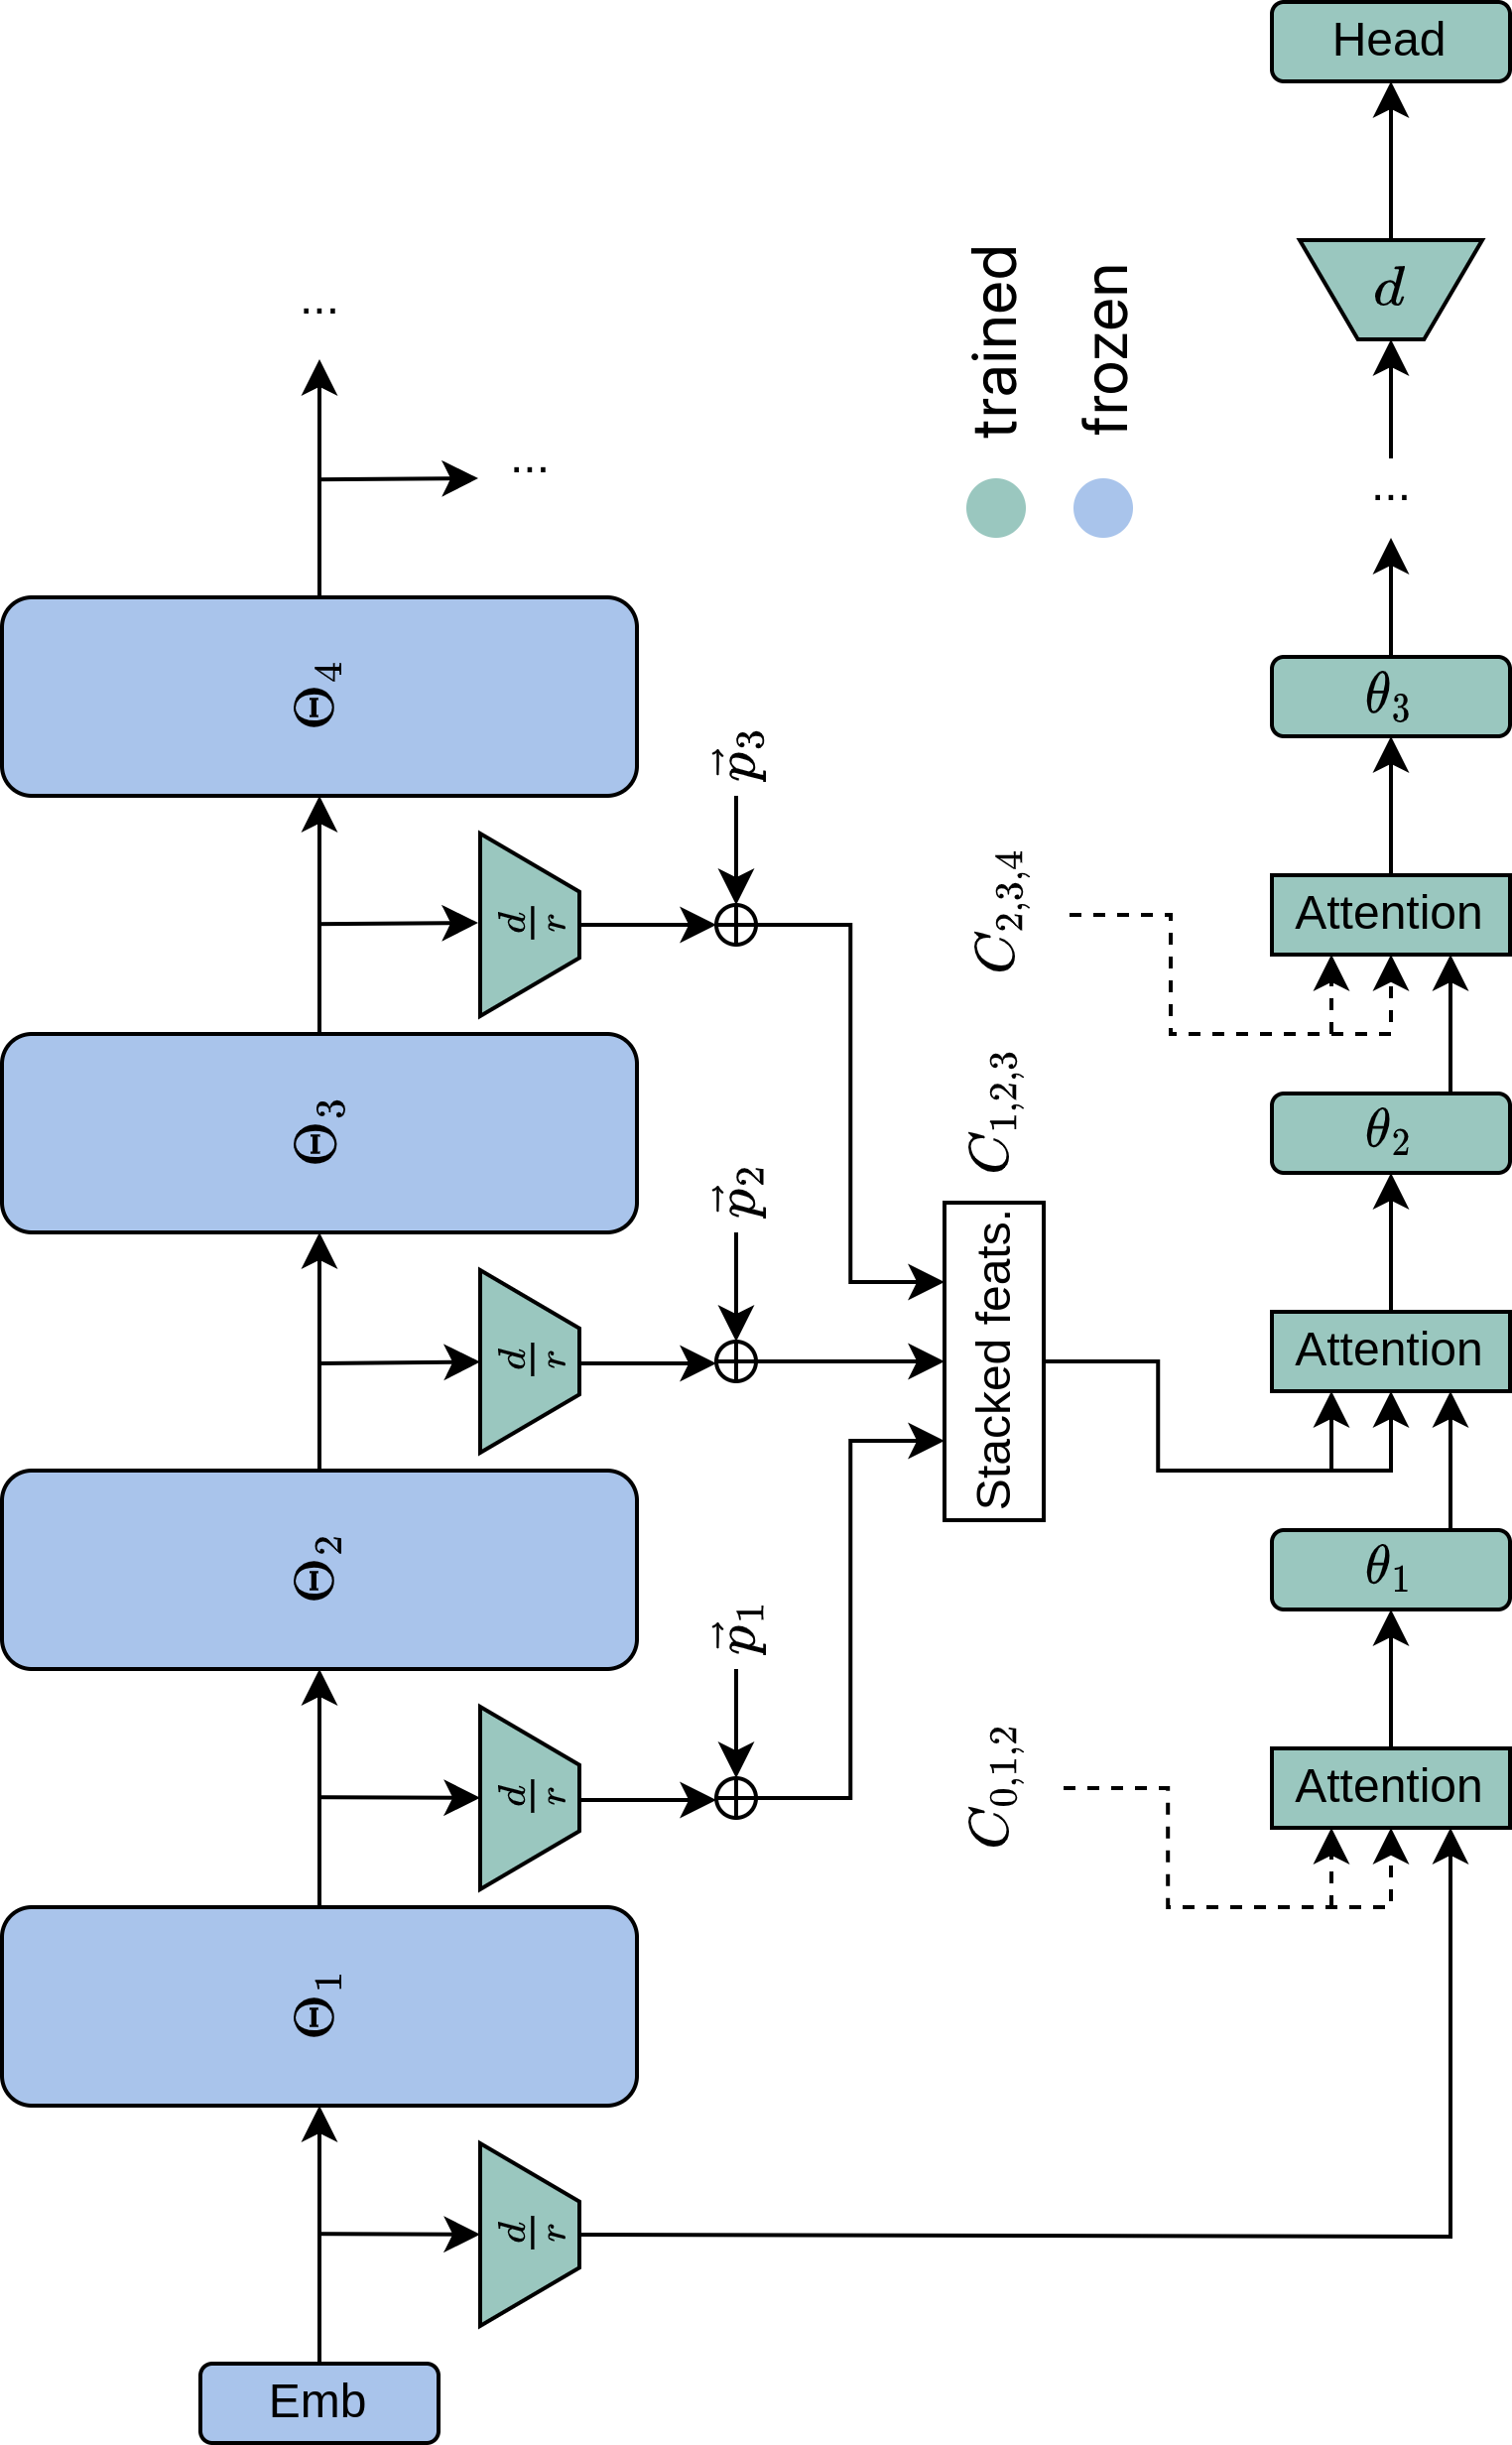
\includegraphics[width=0.4\textwidth, angle=-90]{assets/images/k-LST.png}
    %\includesvg[width=0.5\textwidth, angle=-90]{assets/images/k-LST.svg}
    \caption{This figure shows the k-LST diagram for \(k = 3\). Only the added parameters and head are trained (shown in green), while the backbone remains frozen (shown in blue). We first downsample each feature with a linear projection, before adding the positional encoding and concatenating the features into a single matrix. The features are queried with cross attention by the side network. The backbone's forward pass is completely independent from the side network. The gradients of the trainable parameters can be computed without going through the backbone, resulting in large memory savings.}
    \label{fig:k-LST}
\end{figure*}


\subsubsection{Optimal Hyperparameters}\label{section:lst-parameters}

k-LST has three main hyperparameters: the window size \(k\), the reduction factor \(r\) and the feature dropout probability \(p\). These three parameters provide granular control over the trade-off between memory footprint and performance. A window size of \(k = 9\) showed to be the best performing in our tests. We observed that a higher \(k\) is more susceptible to overfitting. Therefore, for the \(k = 9\) case, we use a feature dropout probability of \(p = 0.2\), while for other experiments we use no dropout. All experiments use a reduction factor \(r = 8\). 9-LST is trained with linear LR decay with warmup. The peak LR is \(\eta = 0.0002\) with a linear decay to \(\text{{2e-6}}\) over \(5\) epochs and a warmup ratio of \(0.12\). All experiments use the AdamW optimizer \cite{DBLP:journals/corr/abs-1711-05101} and the RoBERTa-large \cite{roberta} backbone.


\subsubsection{Benefits for Large Scale Deployments}

The backbone model is completely independent of the side network. This is in contrast to other widely used PEFT methods where the forward pass of the backbone network is directly influenced by the added PEFT parameters. This is a desirable characteristic for large-scale deployment when many different fine-tuned versions of the same backbone model are being served simultaneously. The benefit is derived from the fact that the forward pass of the large backbone model remains constant, regardless of the fine-tuned version. This allows for the batching of requests irrespective of the specific fine-tuned versions. It's a one-way relationship, where the side network has no effect on the output of the backbone model. It simply consumes the intermediate features to produce the final result. As a consequence, there is no need to clone (or dynamically alter) the backbone model. Instead, all requests can pass through the same static backbone model, before the intermediate features are fed into the smaller side networks which can run on smaller compute nodes.
